\subsection{Mechanism overview}
In conclusion, the nD-Laplace mechanism is capable of providing $\epsilon-d_x$-privacy (as well as \gls{gi}) as demonstrated in Formula \ref{theorem:nd-laplace}. The grid-nD-Laplace variant also offers the same privacy guarantee, as proven in Section \ref{section-grid-remapping}. Additionally, the density-nD-Laplace mechanism, being a post-processing step, provides an equivalent level of privacy as nD-Laplace. This equivalence extends to clustering as well.

Furthermore, it is worth noting that the use of kd-trees simplifies the complexity of these variants without compromising their privacy guarantees. Kd-trees serve as a tool to address the search complexity in handling n-dimensional data, rather than directly affecting the privacy assurances.
The following sections will provide a comprehensive framework overview and offer practical insights for its application.

\subsubsection{Flowchart}
\todo[inline]{Check for correctness with truncation/grid-remapping}
All formulas and theories are established for 2D, 3D, and nD-Laplace, so the mechanism design applies to all three variants:
\begin{figure}[h]
  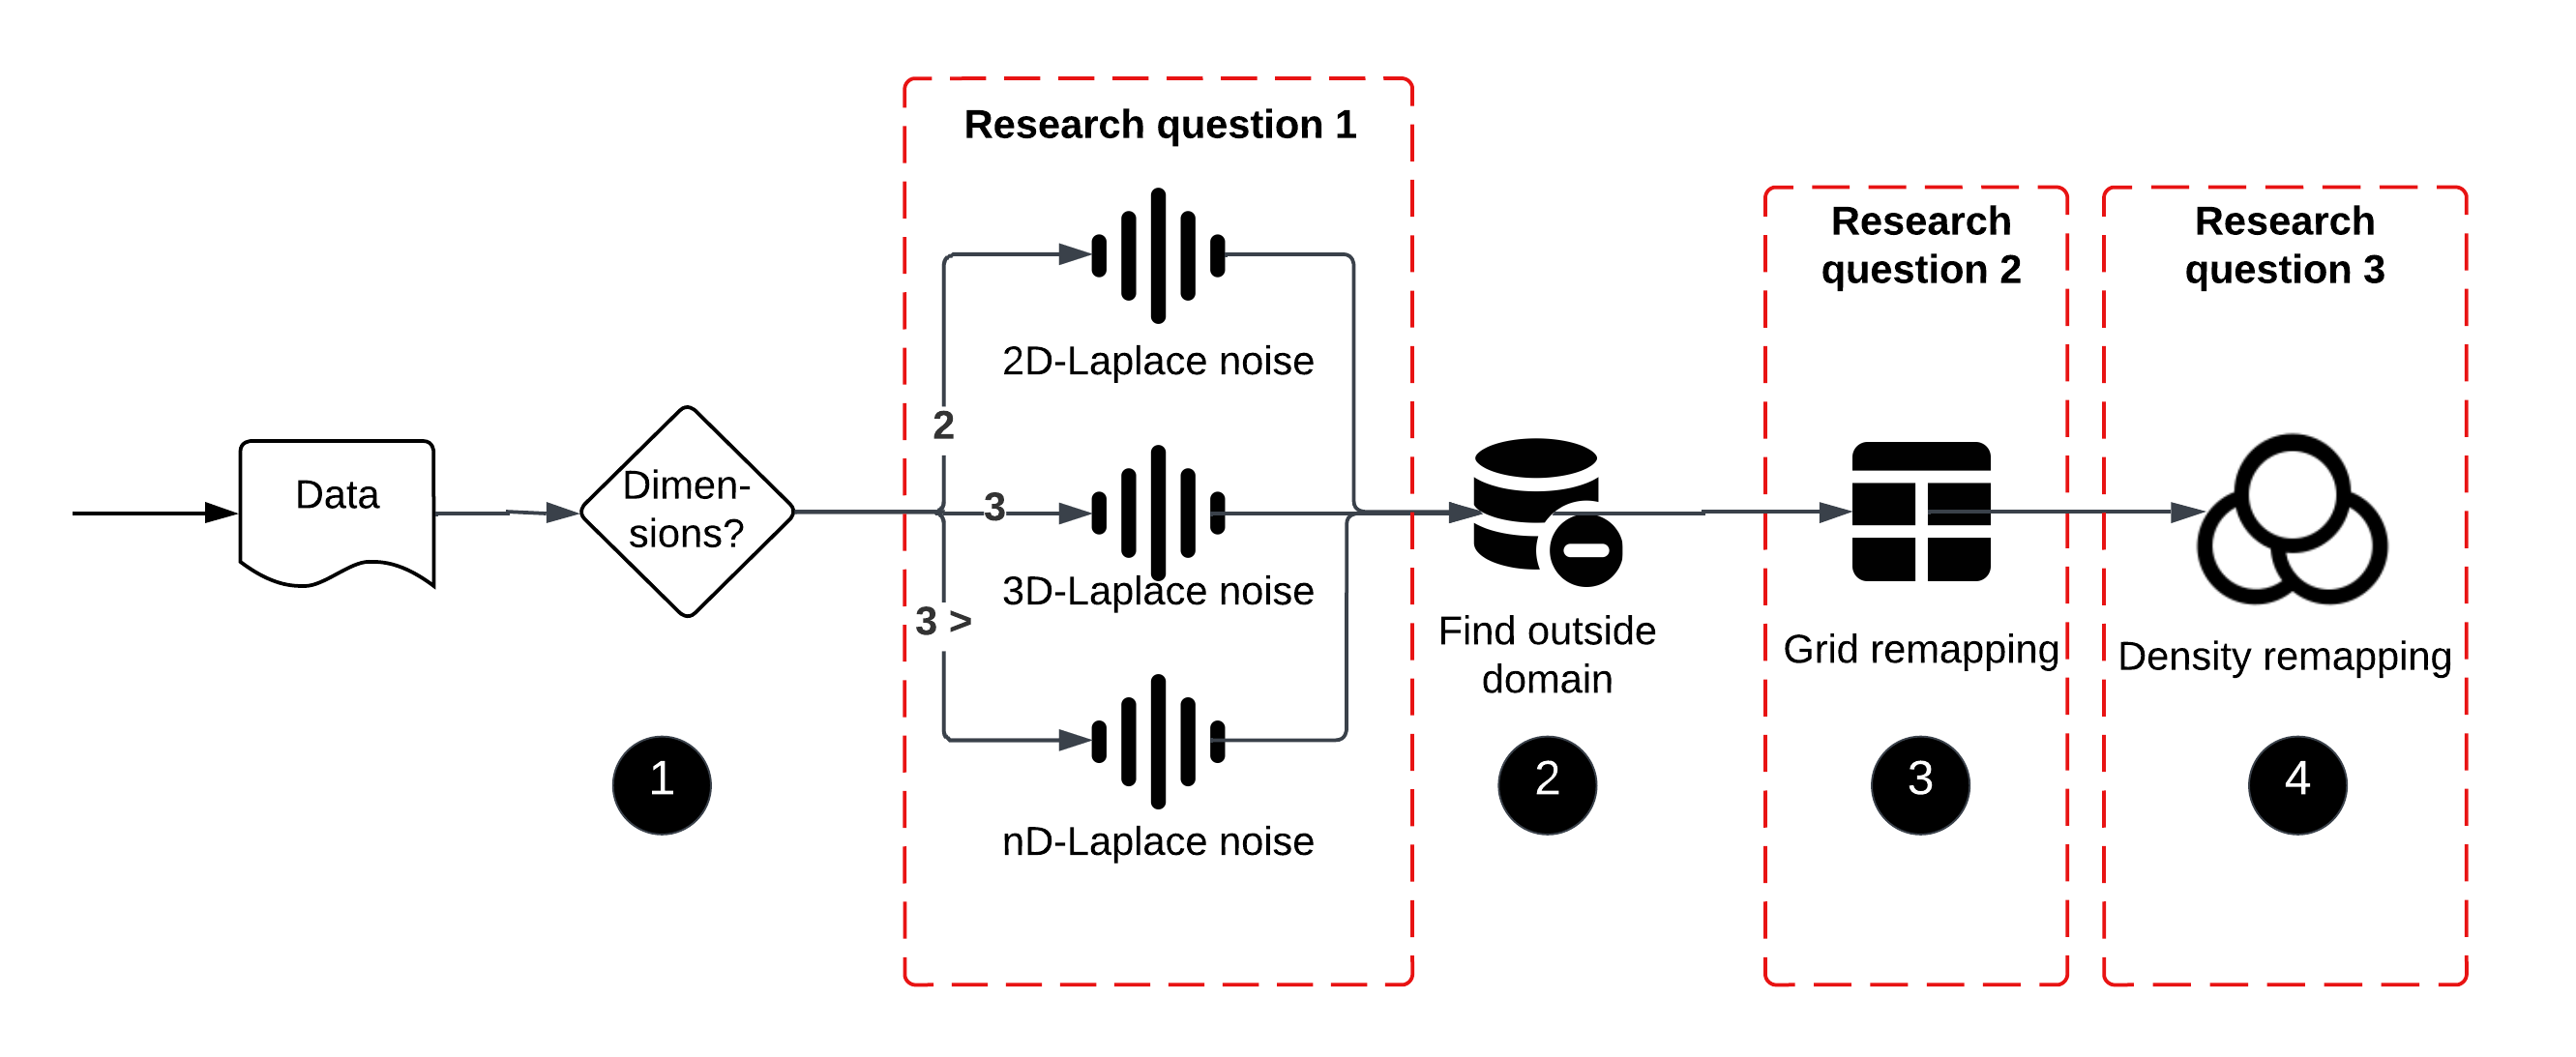
\includegraphics[width=1.1\textwidth]{TheorethicalFramework//ND-Laplace//Images/Thesis-nd - final-mechanism-design.png}
  \caption{Non-interactive mechanism design for nD-Laplace.}
  \label{fig:final-mechanism-design}
\end{figure}
%\todo[inline]{Modify to density-nD-Laplace \& nD-Laplace for image reporting}
For easy navigation, we provide a list of all algorithms:
\begin{enumerate}
  \item Based on the number of dimensions, the algorithm decides the correct Laplace mechanism to use:
        \begin{itemize}
          \item 2D-Laplace:  \ref{alg:2d-laplace}
          \item 3D-Laplace: \ref{alg:3d-laplace}
          \item nD-Laplace: \ref{alg:nd-laplace}
        \end{itemize}
  \item Find points outside domain: \ref{alg:find-outside-domain-laplace}
  \item Grid remapping: \ref{alg:grid-remapping-laplace}
  \item Density remapping: \ref{alg:optimal-remapping-laplace}
\end{enumerate}
In addition, relevant research questions are incorporated into the architecture overview.
These questions are covered in chapter \ref{chapter:methodology}.
\subsubsection{Practical example}
The shape of the dataset is necessary for the usefulness of clustering.
With our algorithm, there are four different shapes/variants of the dataset.
For example, this has been visualized using a 3D dataset based on the heart dataset (\ref{datasets-section}).
Our mechanism aims to provide privacy and preserve the dataset's shape to benefit the utility of clustering.
Grid remapping and optimal remapping are used to achieve this goal.

\begin{figure}[H]
  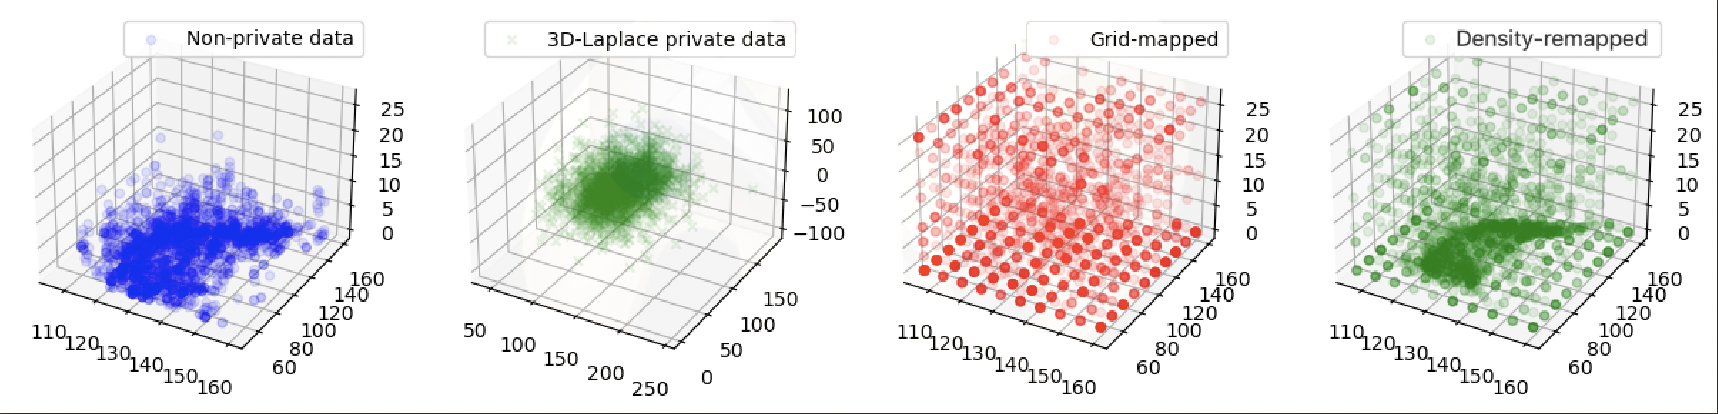
\includegraphics[width=1.1\textwidth]{TheorethicalFramework//ND-Laplace//Images/optimal-remapping-example-2.png}
  \caption{Example of optimal remapping for the 3D-dataset: Cardiotocography. The example shows the different steps of the mechanism in sequence for a dataset perturbed with a privacy budget of 0.1.}
\end{figure}
\begin{enumerate}
  \item Dataset: the blue dots represent the original dataset without any modifications.
  \item Adding noise: the green crosses represent the dataset after adding noise; for this particular example, this is 3D-Laplace (Algorithm \ref{alg:3d-laplace}):
        As can be observed, the data is generated from the center, causing many data points to fall outside the original domain of the dataset.
  \item Grid-remapping: the red dots represent the dataset after grid-remapping (Algorithm \ref{alg:grid-remapping-laplace})
        After performing the grid remapping algorithm, all points within the domain are plotted.
        However, the original shape of the data is mostly lost.
        This makes it challenging to cluster the data as was possible with the original data.
  \item Optimal-remapping: the green dots represent the dataset after optimal-remapping (Algorithm \ref{alg:optimal-remapping-laplace}).
        After completing the previous step, the data points are again remapped based on the (original) density.
        This results in restoring the original shape of the data and, consequently, the clusters.
\end{enumerate}
